\documentclass[a4paper,9pt]{article}
\usepackage[utf8x]{inputenc}
\usepackage[dvips]{graphicx}
\usepackage{fullpage}
\usepackage{simplemargins}

%opening
\title{NGRT4N Documentation}
\author{(c) ITSoftbyrc.com, Inc.}

\begin{document}
%\setallmargins{2cm}
\setcounter{secnumdepth}{4}
\setcounter{tocdepth}{4}

\maketitle


\chapter{Introduction}
NGRT4N is an enterprise-grade IT monitoring dashboard tool that enables IT administrators to build various sorts of synthetic monitoring views. Such views can be used by operators in order to be more efficient in large operational environments such as data centers and Network Operations Center (NOC). Indeed, they enable them to get instant view on the health of the monitored platform, while being able to get more detailed information on each individual component. NGRT4N can work upon different monitoring solutions, which currently include Nagios, Groundwork, Centreon, Icinga, and most of Nagios-derived solutions.

This document is intended to provide you with resources to understand, install and set up, and use NGRT4N. 
%\tableofcontents

\chapter{Overview of NGRT4N}
NGRT4N comes to cover the difficulty to effectively highlight critical events when monitoring in operational environments. Indeed, when the monitored infrastructure grows, the amount of components to check/monitor along with the number of items to observe grow too. When critical events occurred, you have to be able to quickly evaluate their impact on your businesses so to prioritize the recovery of events that have higher impacts. Additionally, it may be useful to show some events to certain users or operators that can address them quickly.  This requires that the monitoring solution enables capabilities of building and manipulating synthetic and dynamic monitoring views. NGRT4N is intended to provide such capabilities.

\section{Prioritized Incident Recovery} %: Effective Monitoring Views and Dashboards
When monitoring in large NOC or data center, it is important that IT organization be able to prioritize incidents based on business impact and more quickly restore services to operation. Using hierarchical views would be a tangible way to effectively achieve such a goal by monitoring high level components such as business processes and services provided to end-users. Indeed, given a service platform consisting of a set of physical and applicative components, a hierarchical organization provides operators with maps that permit them to have a dynamic-consistent view on the health of the platform along with each of its components. 
%This eases the monitoring of IT infrastructure components (systems, applications, network devices, indicators, metrics, etc.) according to their impacts on business processes or end-users.

In order to build relevant hierarchical views, you need to identify the main business process or end-user service along with business processes that will comprise it. Then, you have to link the business processes among them within a hierarchy. Finally, at the bottom level business processes should be related to operating systems, applications, devices, etc. An example of such an organization is illustrated on the figure below. 
In the hierarchy, we differentiate two kinds of nodes according to their relation with native monitoring data collected by the monitoring engine:
\begin{itemize}
 \item {\bf Native Check (NC)}: Such nodes are directly linked to a basis check (process check, load check, http check, etc), and are located at bottom of the hierarchy (sheet nodes).
 \item {\bf Business Process (BP):} This kind of nodes consists of structural nodes that you or your administrator can define in order to meet monitoring requirements. They consist of high level systems (e.g. operating system, device, application tier, etc.), business processes (e.g. notification, authentication, smtp, etc.), services provided to end-users (hosting, download, SMS, MMS, etc.) and so forth. Located at a higher level than native-check nodes within the hierarchy, they can have one of more child items which can be both native-check or business-process nodes. {\bf IMPORTANT:} All the sheet nodes of a hierarchy have to be native checks in order to ensure the consistency of the related monitoring view.   
\end{itemize}
%The items retrieve to monitoring database are located on the bottom of the hierarchy and can not have any sub-item. Other items located in a higher level in the hierarchy are business process, application service, service provided to end-users, etc. %Their statuses are updated according to the status of the status data collected by the monitoring engine. 
\begin{figure}
\centering
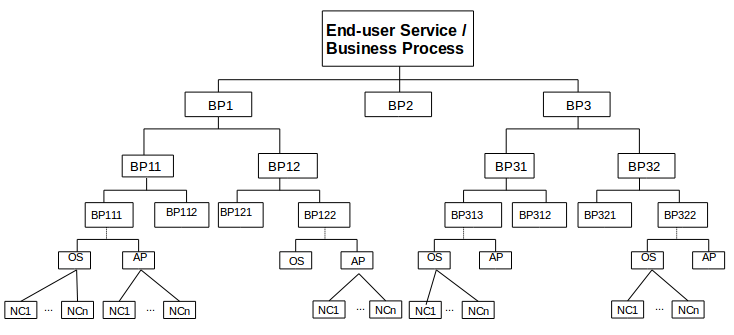
\includegraphics[width=12cm]{images/hierarchical-mv.png}
\caption{An illustration of hierarchical organization to monitor a given business process or service}
\end{figure} 

Each monitoring view hierarchy is defined through a configuration file, in which each node is defined by a set of properties that permit to identify it along with its possible child nodes. The MVB utility of NGRT4N provides functionally that ease the creation and the edition of such  configuration files. It maintains the structure of the hierarchy (relationship among nodes) internally and transparently to user. The following list describes the properties that user has to edit when editing a node.  

\begin{center}
        \begin{tabular}{p{3cm} p{3cm} p{20cm}}
        {\bf Property} & {\bf Applicability} & {\bf Description}\\
        Name & ALL & REQUIRED, this parameter provides a short name to the node. Used like label when representing or referencing the node on the operator console, its value can be for example, the name of device, system, application, business process, end-user service, etc. \\ 
        Type & ALL & REQUIRED, the type property can be either \emph{Native Check} or \emph{Business Process} (default value).\\ 
        Status Aggregation Rule & Business Process & REQUIRED, this parameter specifies the rule to use to update the status of the node according to the statuses of its child nodes.\\
        Icon & ALL & REQUIRED, the icon property specifies the name of to use to represent the the node on the hierarchy map. The user has to select an images among a list of built-in icons, otherwise the default icon (representing a business process) will be used.\\
        Description & ALL & OPTIONAL, this field holds a text that provides a more-descriptive information about the node. \\ 
        Alarm Message & Native Check & OPTIONAL, this field holds a text message to show on event console when the state of the node becomes abnormal (when a critical or major event arises on the node). If there is not any message specified, the default message provided by the monitoring engine will be used. \\
        Notification Message & Native Check & OPTIONAL, this field holds a text message to show on event console when the state of the node (is) becomes normal. If there is not any message specified, the default message provided by the monitoring engine will be used.\\
        Related Native Check & Native Check & REQUIRED, this property holds the identifier of the monitoring data (collected  by the monitoring engine) to link to the node.\\
        \end{tabular}
\end{center}

%The MVB utility of NGRT4N provides functionally that ease the creation and the edition of such  configuration files. It maintains the structure of the hierarchy (relationship among nodes) internally and transparently to user. Editing such files from a text editor could be not easy. In particular, it could be tricky to maintain the relation among components (nodes), especially when their number grows. 

\section{Features and Benefits}
The following list describes the major features and benefits of NGRT4N:

\begin{description}
        \item [Hierarchical Business Process Monitoring]
        Using NGRT4N, your network administrators can build hierarchical monitoring views to monitor platforms consisting of individual (or set of) business process(es) or end-user service(s). Such monitoring views allow operators to quickly evaluate the real impacts (on your business activities) of critical events that can arise on systems, applications, devices, etc.     
        \item [Comprehensive Monitoring]
        NGRT4N permits the customization of messages shown on operator console. This enables operators to get more comprehensive messages when needed, instead of the monitoring engine native output which can be crabbed. For example, instead of getting a message like \emph{"DISK CRITICAL - free space: / 5483 MB (28\% inode=67\%)"} on your console (according to the Nagios plug-in), you can have a more comprehensive message like \emph{"The free space available in the server <hostname/IP> root partition is less than 30\%"}.
        \item [Interactive Dashboard at a Glance]
        NGRT4N provides intuitive, friendly and easy to use graphical user interfaces (GUI). Being interactive, they allows operators to get real-time overview on the health of the monitored platform, while being able to quickly get more detailed information on the collected monitoring data (metrics or checks on systems, applications, devices, etc).  
        \item [Monitoring View Builder] 
        NGRT4N provides an utility that enables administrators to build the configuration of monitoring views. They can easily select the data to retrieve from the whole ones collected by the monitoring engine, set (when needed) the messages to show on event console upon the appearance of a given event, etc. Thank to "drag-and-drop" that enables hierarchy reorganization advanced-capabilities.
        \item [Secure Access to Monitoring Data]
        The access to monitoring data through NGRT4N is subjected to two authentication mechanisms. Being a X application, NGRT4N is typically deployed on the monitoring server and used through a ssh-tunneled X forwarding mechanism. This permits to leverage the improved security capabilities enabled by SSH, in addition to its built-in authentication mechanism . 
        \item [Support of Various Monitoring Solutions] 
        NGRT4N has been tailored to be loosely coupled with the underlying monitoring solution so to adapt to  various monitoring solutions. It currently supports Nagios, Groundwork, Centreon, Icinga, and most of Nagios-derived solutions.
\end{description}


\section{User Interfaces}
NGRT4N consists of two main utilities or programs: the \emph{Operator Console} and the \emph{Monitoring View Builder}.

\subsection{Operator Console}
The GUI of the Operator Console (OC) is depicted on the Figure below. This interface is easy to use and provide the following functionality:
\begin{itemize}
        \item An event console shows the messages specific to the monitored platform.
        \item The Explorer Pane and the Dashboard Tab respectively contain a tree and a map of the monitoring view hierarchy. These different representations permit to view, explore, and manipulate the view in friendly and interactive way without limit on its hierarchy's depth.
        \item The Chart Panel gives an overview on the health of the monitored platform.
        \item Menus (tool-bar and context menus) along with mouse-wheel event handling permit to easily explore the graph in order to get detailed information. It is possible to zoom (out and in) to reach a given item or region, jump to a given item, or filter messages related to a given item and its sub items. 
        \item The Native Web UI Tab is an embedded web browser that allows operators to get access to the default web interface of the monitoring solution, if any. 
        \item User is also able to change the url loaded in the web tab, change the interval of updating the console, capture a picture of the dashboard, change its password, get the online documentation, etc.
\end{itemize}

\begin{figure}
\centering
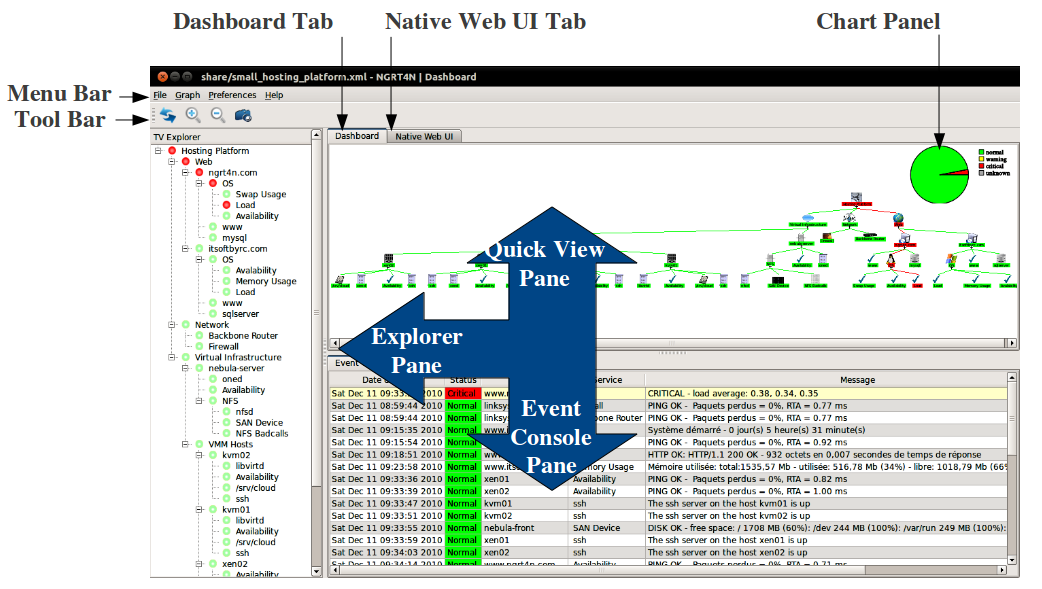
\includegraphics[width=18cm]{images/annotated-dashboard.png}
\caption{NGRT4N's Operator Console showing an example of monitoring view}
\end{figure}

\subsection{Monitoring View Builder}
The GUI of the Monitoring View Builder (MVB), depicted on the Figure below, is powerful interface that allows users to easily create or edit the configuration of monitoring views. It consists of two main panes (the Explorer Pane and the Edition Pane) and provides the following functionality: 
\begin{itemize}
        \item On-the-fly adding of sub items (child node-items) of a given monitoring view hierarchy node-item.
        \item Drag-and-drop alteration of the hierarchy without limit on the depth of the hierarchy.
        \item Easy selection of the monitoring data (check or metric) to link to a given node item. They can be selected either directly through their identifiers or from a selection list.
        \item Set custom messages to show on event console upon events appearance. Each message can have specific tags that will be replaced in order to contextualize the message (with the associated component name) before showing it on console.   
\end{itemize}

\begin{figure}
\centering
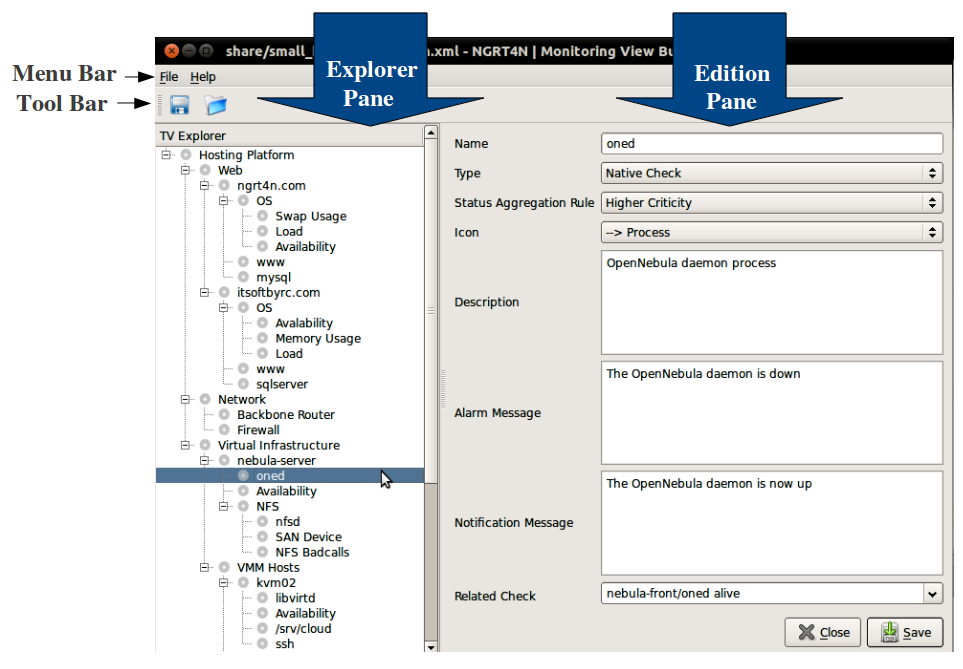
\includegraphics[width=18cm]{images/annotated-editor.png}
\caption{NGRT4N's View Builder showing the editing of a given monitoring view item}
\end{figure} 

\chapter{How NGRT4N Fits in a Monitoring Environment}
In this section we briefly introduce the design of NGRT4N to show a suitable architecture for integration in a preexisting or new monitoring environment. 
 
\section{Architecture of Integration}
In order to reduce the integration constraints, NGRT4N is designed to be loosely coupled with the monitoring solutions and any other tool. As introduced on the Figure below, it architecture relies upon the database of status data collected by the monitoring engine. In the case of Nagios-derived solutions such as Nagios it self, Centreon, Groundwork Monitor, Icinga, etc., NGRT4N only needs to get access to the file named \emph{status.dat}.

\begin{figure}[!t]
\centering
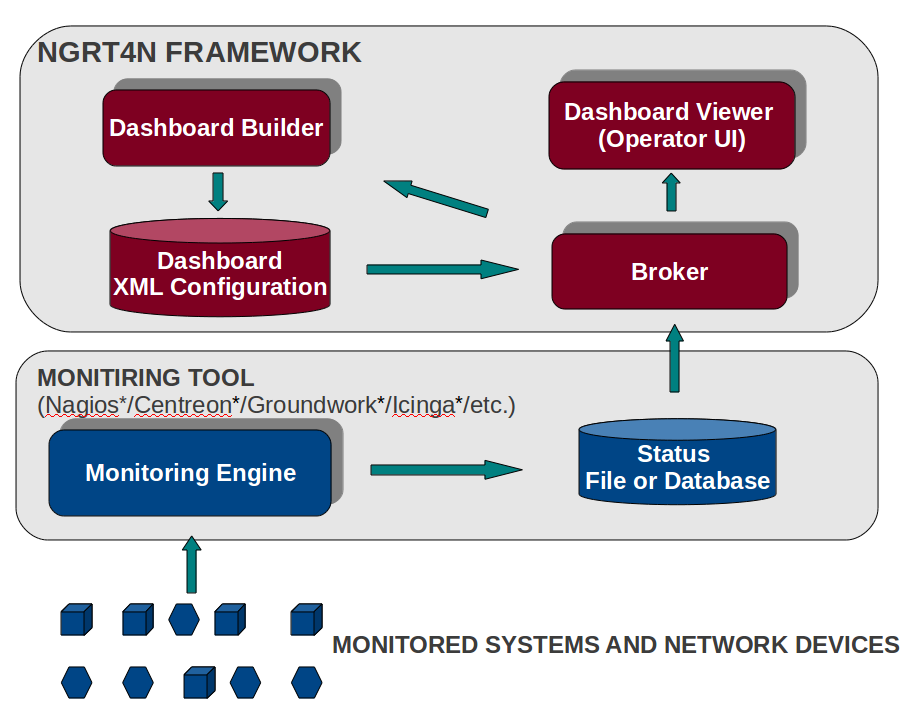
\includegraphics[width=10cm]{images/software-integration.png}
\caption{Architecture of NGRT4N fiting with the monitoring solution}
\end{figure} 
%Each monitoring view is represented with a single configuration file that contains the set of data to retrieve in order to update the view.

NGRT4N is coupled with the monitoring solution through an internal solution-aware \emph{Broker}. The broker is in charge to access the status database periodically to retrieve the status data in order to update monitoring views. The default value of the updating interval is five minutes, but it can be changed by administrators to suit your monitoring needs. 

When the coupling with the monitoring database is suitable configured, the MVB (Monitoring View Builder) can retrieve the list of checks from this database in order to ease the selection of items to link to monitoring view. This is useful to avoid erroneous selections due to invalid references to check identifiers.


\section{Access to User Interfaces}
NGRT4N assumes that your physical infrastructure adopts a classical monitoring architecture with a monitoring server, a set of monitored systems and devices, and workstation where user operates). 

\begin{figure}
\centering
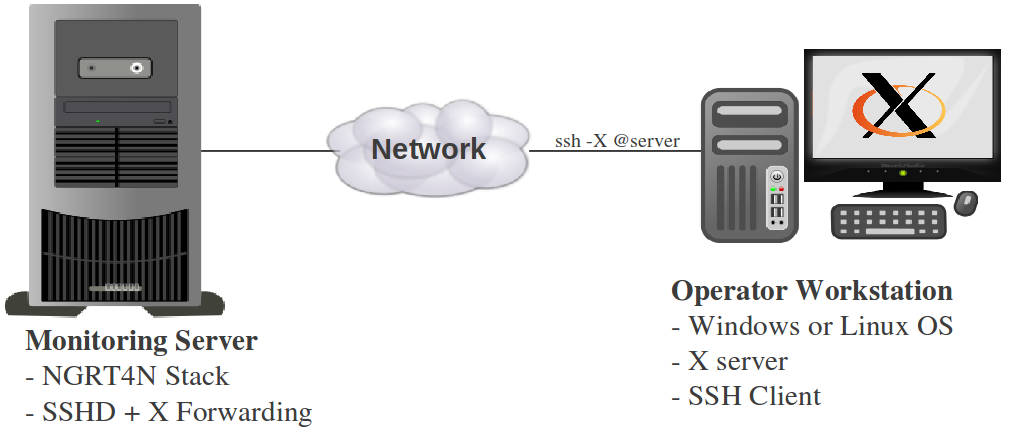
\includegraphics[width=12cm]{images/physical-integration.png}
\caption{Typical architecture for integrating NGRT4N within a monitoring environment}
\end{figure}

In this architecture, the NGRT4N stack is installed on the monitoring server and is accessible to users (on workstations) via a X forwarding mechanism. In order to be secure, the X forwarding has to work through a ssh tunnel between the monitoring server and the operator workstation. This requires to activate X forwarding either in the ssh daemon (by setting \emph{ForwardX11 yes} in \emph{/etc/ssh/ssh\_config}) or from the ssh connection command (\emph{ssh -X @server} or alternatively by setting \emph{ForwardX11 yes} in \emph{\$HOME/.ssh/config}) from the workstation.   



\chapter{Getting Started with NGRT4N}
This section is intended to provide you with simple instruction on how to install and use NGRT4N.

\section{How to Get NGRT4N}
Check the NGRT4N Home Page at http://www.ngrt4n.com for information about the current version and for downloading instructions.

NGRT4N is distributed as pre-compiled binary packages. 

\section{System Requirements}
\label{systemreq}
\subsection{Monitoring Server}
NGRT4N is designed to work on Linux systems. 
Its installation does not have additional requirements, but it requires some third-party libraries at runtime:
\begin{itemize}
\item {\bf Qt >= 4.6}. At least the following modules should be installed: {\bf QtCore, QtGui, QtNetwork, QtWebkit, QtXml, QtXmlPatterns}. 
\item {\bf Graphviz >= 2.20.2}. At least the {\bf dot} utility should be installed. NGRT4N has been tested with graphviz 2.20.2, but it may work on former versions.
\item {\bf ssh}
\item {\bf xauth}
\end{itemize}

Most of Linux distributions provide these libraries as pre-compiled packages. They may be already installed on your system, check before proceeding to a new installation. If there are not installed, you can install them from the package manager (yum, apt-get, synaptic, etc.).  
You don't need to care about qt dependencies if you have downloaded one of the large distribution packages of NGRT4N.

\subsection{Operator Workstation}
NGRT4N can be run from any system having the following software installed:
\begin{itemize}
\item {\bf ssh client}. On Linux and MAC OS systems, a ssh client should be already installed. On Windows, you may need to install a ssh client such as {\bf PuTTY}
\item {\bf X Server}. On Linux and MAC OS systems with graphical interfaces, a X server should be already installed. On Windows, you may need to install a X server such as {\bf Xming}
\end{itemize}

\section{Hardware Requirements}
\subsection{Disk Requirements}
The installation of NGRT4N requires a small disk footprint, less than less than 50MB of free disk space is required for installing a large distribution along with its dependencies (Qt libraries and graphviz binaries). A small amount of disk space is required to store the configuration of monitoring views. E.g. Less than 100KB are required for a view with more than 500 components. 

\subsection{Memory Requirements}
256 MB of free space in physical memory and could be a good starting point. However the amount of required memory at runtime obviously depends on the number of operator consoles running in parallel, as well as on the amount of nodes that constitute the views loaded on those consoles. However, we recommend to continuously check your server to ensure that it still responds well after changing one or more of these parameters.

\subsection{CPU Requirements}
The CPU requirements depend on the number of operator consoles running in parallel, the intervals of updating those consoles, and the amount of items to retrieve to the monitoring database at each update. E.g. For an update interval of 5 minutes, 1 CPU core can be sufficient to update up to 5 operator consoles, which each deals with about 100 items retrieved from monitoring database at each update. However, we recommend to continuously check your server to ensure that it still responds well after changing one or more of these parameters.

\section{Installation}
The installation of NGRT4N is a straightforward task. In most of cases, less than 10 minutes are required to make it ready to use.

During the installation you'll need to have {\bf root} access to your machine.

\paragraph{Installing Runtime Pre-requisites}

On the monitoring server and operator workstations, make sure that all runtime pre-requisites (\ref{systemreq}) are installed.

\paragraph{Download NGRT4N}

Check the NGRT4N Home Page at http://www.ngrt4n.com for information about the current version and for downloading instructions.

NGRT4N is distributed as pre-compiled binary packages. 

\paragraph{Install NGRT4N}

Extract the NGRT4N binary tarball.

tar zxf ngrt4n-X.Y.Z.tar.gz

cd  ngrt4n-X.Y.Z

Run the NGRT4N install script. 

./install.sh 

NGRT4N works in a self-contained directory, by default /opt/ngrt4n. You can change this location using the -d switch (./install.sh -d <destination_folder>. 

\paragraph{User Information}
NGRT4N distinguishes two types of user profiles: a \emph{operator profile} and a \emph{administrator profile}. An operator can create, edit, and view monitoring views, whereas an administrator can have more control such as defining monitoring settings (update interval, path to status database, etc.).

There are two predefined users associated to these profiles.

Operator User

{\bf Login:} ngrt4n\_op

{\bf Password:} nrt4n\_op     (You need to change this as soon as possible)

Administrator User

{\bf Login:} ngrt4n\_adm

{\bf Password:} ngrt4n\_adm     (url for accessing to the native web interface of monitoring)

\paragraph{Configuring NGRT4N}

Once installed NGRT4N users should have the following environments variables set as follows:
 
\begin{center}
        \begin{tabular}{p{4cm} p{20cm}}
        NGRT4N\_HOME & This variable must be set to \emph{/opt/ngrt4n} or \emph{<destination\_folder>} if have used the -d option at installation time. \\
        PATH &  \$NGRT4N\_HOME/bin:\$PATH
        \end{tabular}
\end{center}

Run the configuration wizard and log on as administrator to set suitable monitoring settings, and change the default password.

ngrt4n -c

We mention that NGRT4N is a command line tool consisting of one main program named \emph{ngrt4n}. There are options to launch its different modules. Run ngrt4n -h to have the list of available options and their usage. 

\paragraph{You're Done}
Congratulations! You successfully installed NGRT4N. You'll no doubt want to see it in action, so check out the following tutorials.

\section{Tutorial}
This tutorial describe how you can use NGRT4N to create the configuration of a view based on hierarchical business processes to monitor a given service platform. You will first use the VCE utility to edit the view configuration file and then, load this file with the OC utility.

In order to make this tutorial fluid, we will proceed by showing NGRT4N in action from a case study example. 

\subsection{Case Study}
Once NGRT4N installed, you should have example files located in {\bf \$NGRT4N_HOME/share/examples}. The configuration of view are stored in xml files (.xml). We will use the example named {\bf small_hosting_platform.xml}, which works with the status database {\bf status.dat} located in the same directory. This is an illustration of a platform monitored by Nagios. The platform is used to provide web hosting to end users. It relies on virtualized resources and provides web access from two servers.

Connect to the server where is installed NGRT4N, and run the configuration utility.

ssh -X user@server

ngrt4n -c

Log on as administrator, and point the status database to \$NGRT4N_HOME/share/examples/status.dat. You can also change the update interval. Leave the url of the web interface unchanged, or point it to your monitoring web interface. 

Apply change and quit the utility.

\subsection{Use the OC Utility}
In order to show the view with the OC utility, run the ngrt4n program with the -d switch while specifying the configuration file to load. 

ngrt4n -d \$NGRT4N_HOME/share/examples/small_hosting_platform.xml

The example show a case where a critical event has arose on a web server. According to its criticality on the platform the hierarchy has been configured so to propagate the criticality unchanged until the top of the hierarchy. However, as we will show in the next sub section this behavior can be changed by modifying the \emph{Status Aggregation Rule} property of one or more of its ascendant nodes when editing the view.

You can play with the view to see the powerful of NGRT4N. Each item in the hierarchy map and the three view explorer has a context menu and a tooltip. You can zoom the hierarchy map using the suitable menu from either the toolbar or the menu Map. Alternatively you can use the mouse wheel. Go through menu to test other functionalities, such as capture an image of the current view of the hierarchy map, hide the statistics chart, change the user password, show monitoring settings and change them if needed (only administrator), etc.

\subsection{Use the VCE Utility}
We have shown how hierarchical view could be relevant to manage incidents in monitoring environments. Now we will show how such a view can be easily created and edited from the NGRT4N's VCE utility, which is executed using the -d option. 

\end{document}
